\documentclass[xcolor=dvipsnames, compress, t]{beamer}

\usetheme{CambridgeUS}
\usepackage[english]{babel}
\usepackage{color}
\usepackage{graphics}
\usepackage{graphicx}
\usepackage{stmaryrd}
\usepackage{etoolbox}
\usepackage{multicol}
\usepackage{tikz}
\usetikzlibrary{shapes.geometric, arrows}

\usepackage{dsfont}
\usepackage{etoolbox}
\usepackage{accents}
\usepackage{sgame}
\usepackage{epstopdf}
\usepackage{wrapfig}
\usepackage{tabto}

\setbeamertemplate{theorems}[numbered]
\undef{\lemma}
\newtheorem{lemma}{\translate{Lemma}} %gives own numbered lemmas
\newtheorem{prop}{Proposition}
\newtheorem{defin}{Definition}
\newenvironment{sketch}[1][Sketch of Proof.]{ \begin{trivlist} \item[\hskip \labelsep {\bfseries #1}]}{\end{trivlist}}

%colors

\definecolor{NIUred}{RGB}{200,16,46 } 
\definecolor{NIUblack}{RGB}{0,0,0}
\definecolor{NIUpantone}{RGB}{165,167,168}

\setbeamercolor{palette primary}{bg=NIUblack,fg=white}
\setbeamercolor{palette secondary}{bg=NIUpantone,fg=white}
\setbeamercolor{palette tertiary}{bg=NIUred,fg=white}
\setbeamercolor{palette quaternary}{bg=NIUred,fg=white}
\setbeamercolor{structure}{fg=NIUred} % itemize, enumerate, etc
\setbeamercolor{section in toc}{fg=NIUred} % TOC sections
%\setbeamercolor{subsection in head/foot}{bg=NIUpantone,fg=white}
%%Special Commands
\newcommand\munderbar[1]{%
	\underaccent{\bar}{#1}}

\newcommand{\der}{\mathrm{d}}
\newcommand{\e}{\mathrm{e}}

\newcommand{\vs}{\vspace{\baselineskip}}
\newcommand{\vf}{\vspace{5pt}}
\newcommand{\draw}{{\color{Plum} \bf Drawing.}} 
%use this if there is a drawing that you can't include
\newcommand{\wts}[1]{{\color{Orchid} \textbf{\underline{WTS}:}  #1}} 
%use this for what to show!

\setbeamertemplate{navigation symbols}{} 
\setbeamertemplate{enumerate items}[default]

%%Don't change things above this%%

%%%%%%%%%%%%%%%%%%


\title[691 Presentation]{Demographics and U.S. Presidential Elections}

\subtitle{Can Changing Population Characteristics Explain Elections?}

\author{Ethan Rahman}
\institute[NIU]{\vspace{-10pt} \large Northern Illinois University}
\date{October 15, 2021}

\renewcommand{\thedefin}{4.\Alph{defin}} %ended on 4.C
\setcounter{defin}{3}

\renewcommand{\thetheorem}{4.\arabic{theorem}} %ended on 4.2
\setcounter{theorem}{2}

\renewcommand{\thelemma}{4.\roman{lemma}}
\setcounter{lemma}{0}

\begin{document}
	\begin{frame}
		\titlepage
	\end{frame}
	
	\begin{frame}{States} 
		I was assigned 5 states in the mid-Atlantic region of the United States:
		\begin{minipage}{.25 \textwidth}
			\begin{itemize}
				\item Maryland
				\item Pennsylvania
				\item New Jersey
				\item Virginia
				\item Delaware
			\end{itemize}
		\end{minipage}
		\begin{minipage}{.50\textwidth}
			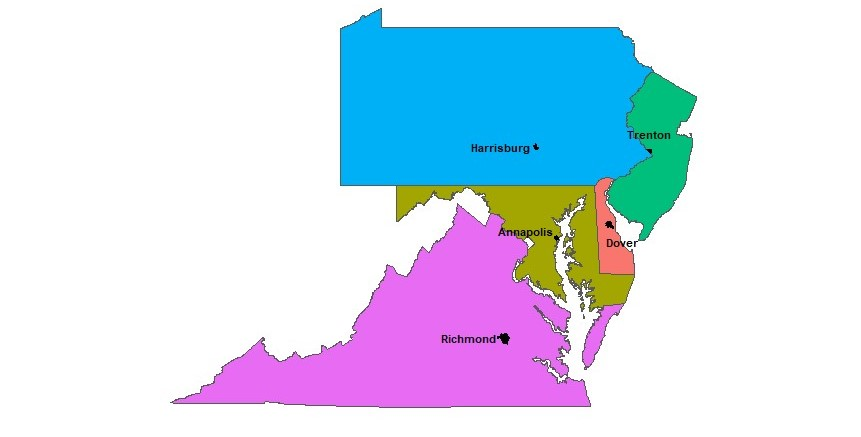
\includegraphics[width=1.8\textwidth]{Rplot03_cropped.jpg}
		\end{minipage}
	\end{frame}
	\begin{frame}{Brief Overview of Each State} 
		\begin{center}
			\resizebox{\textwidth}{!}{%
			\begin{tabular}{ |p{0.16\linewidth}|p{0.16\linewidth}|p{0.16\linewidth}|p{0.16\linewidth}|p{0.16\linewidth}|p{0.16\linewidth}| } 
				\hline
				\multicolumn{6}{|c|}{Mid Atlantic States}		\\
				\hline
				{}           & Maryland & Pennsylvania & New Jersey & Virginia & Delaware\\
				\hline 
				Population   & 6,018,848& 12,791,530   & 8,878,503  & 8,454,463&  957,248\\ 
				Largest City &Baltimore & Philadelphia &Newark  &Virginia Beach& Wilmington\\ 
				Largest Industry (by number of employees) & Real estate&Health Care and Social Assistance &Health Care and Social Assistance & Health Care and Social Assistance & Finance and insurance \\
				\hline
			\end{tabular}}
		\end{center}	
	\end{frame}
	
	\begin{frame}{Quadratic Forms}
		
		{\color{Orchid} $$f(x) = bx^2$$} 
		
		\vspace{-\baselineskip}
		
		\begin{defin}
			A \underline{quadratic form} on $\mathds{R}^k$ is a real-valued function of the form $$Q(x_1, ..., x_k) = \sum_{i, j=1}^k a_{ij} x_i x_j.$$
		\end{defin} \pause
		
		Level curve:  $a_{11} x_1^2 + a_{12} x_1 x_2 + a_{22} x_2^2 = b$
		
		$\rightarrow$ ellipse, hyperbola, pair of lines, empty set (i.e. conic sections) 
		
		{\color{MidnightBlue} Common for econ: indifference curves}\pause
		
		\vs Matrix Representation (``Expansion around a matrix'')
		$$\begin{pmatrix}x_1 & x_2 \end{pmatrix} \begin{pmatrix} a_{11} & a_{12} \\ 0 & a_{22} \end{pmatrix} \begin{pmatrix} x_1 \\ x_2 \end{pmatrix} $$
		
	\end{frame}
\end{document}